\section{Reducing Finite-Event Prediction Error}
\label{app:relinearized-recovery}
\newcommand{\RefineOld}{3.191}
\newcommand{\RefineNew}{0.139}
\newcommand{\RefineFine}{0.0155}
\newcommand{\RefineGain}{95.7}


\begin{figure*}[t]\centering
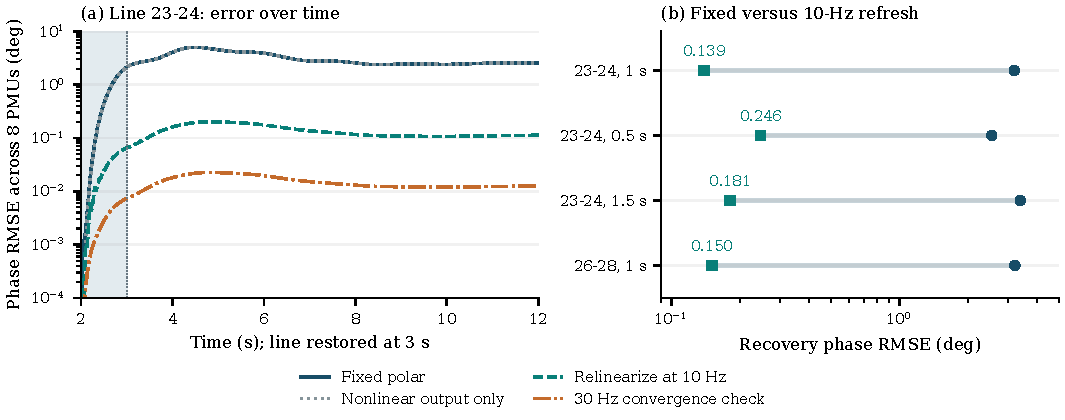
\includegraphics[width=.98\textwidth]{figures/generated/relinearized_recovery.pdf}
\caption{Prediction refinement with known events and no measurement updates.
(a) Phase RMSE across eight PMUs at each report; the shaded interval marks
the active opening. The observation-only control almost overlaps the fixed
predictor. (b) Recovery RMSE over each case's restored interval: circles
use fixed dynamics, squares refresh every three reports. All four line
cases are shown. The finer refresh in (a) checks convergence; it is not
a method selected after inspecting the comparison.}
\label{fig:relinearized-recovery}
\end{figure*}

The preceding line-recovery error motivates a separate predictor comparison.
The hypothesis is that recomputing local dynamics along the predicted
trajectory reduces the error left by a fixed expansion point. This changes
the physical approximation, not the plant, terminal assignment or noise law.

At a refresh time $t_j$, take the predictor's current state as
$x_j=\hat x(t_j)$ and solve $G_q(x_j,z_j,a)=0$. Compute the
mass-normalized field $f_j$ and reduced Jacobian $A_j$ there. Until the next
refresh, propagate the local affine model by
\begin{equation}
 \hat x(t_j+s)=x_j+
 \left[\exp\!\left(s
 \begin{bmatrix}A_j&f_j\\0&0\end{bmatrix}\right)\right]_{1:n,n+1}.
 \label{eq:recentered-flow}
\end{equation}
This expression starts from zero deviation at each new anchor, retains
the absolute predicted state, and requires no inverse of $A_j$.
At every report, solve the algebraic constraints at $\hat x$ and form the
topology-specific voltage and terminal-current observations. A known switch
forces an immediate refresh; differential states are not reset. The new
reference comes entirely from previous model predictions, never subsequent
true internal states or measured corrections. This is local linearization
with nonlinear algebraic observations, not an iterated measurement update.

\subsection{Separate Dynamic and Observation Refinement}
The protocol fixes a refresh every three reports (0.1\,s) before execution.
It compares the fixed dynamics and first-order polar observation of the
preceding section, the same fixed dynamics with nonlinear algebraic
observations, and the refreshed dynamics with those same observations.
A one-report refresh is retained only as a convergence diagnostic.
No interval is selected by minimizing the observed errors.

Seven 12-s trajectories comprise a normal control, the previous bus-7
$\pm10\%$ load changes, the previous 1-s opening of line 23--24, two new
opening durations of 0.5 and 1.5\,s on that line, and a 1-s opening of line
26--28. Each event starts at 2\,s; loads restore at 6\,s. All methods know
the event, its times and the initial condition. All seven nonlinear solves
and all predictor runs succeed, with continuous differential states and
algebraically consistent outputs. These are deterministic development
checks with three prospective line cases, not independent random parents
or a transfer experiment.

\begin{table}[t]\centering\small
\caption{Recovery voltage-phase RMSE (degrees). All methods receive the same known event and initial state. The 30-Hz refresh is a convergence check, not a replacement selected after evaluation.}
\label{tab:relinearized-recovery}
\setlength{\tabcolsep}{3.1pt}
\begin{tabular}{lrrrr}
\toprule
&Fixed&Nonlinear&\multicolumn{2}{c}{Relinearize}\\
Event&polar&output only&10 Hz&30 Hz\\
\midrule
23--24, 1 s&$3.191$&$3.191$&$0.139$&$0.0155$\\
23--24, 0.5 s&$2.542$&$2.541$&$0.246$&$0.0279$\\
23--24, 1.5 s&$3.390$&$3.390$&$0.181$&$0.0203$\\
26--28, 1 s&$3.211$&$3.212$&$0.150$&$0.0169$\\
Bus 7, $+10\%$&$0.119$&$0.119$&$6.6\times10^{-5}$&$7.5\times10^{-6}$\\
Bus 7, $-10\%$&$0.119$&$0.119$&$6.6\times10^{-5}$&$7.5\times10^{-6}$\\
\bottomrule\end{tabular}
\end{table}


The reference line's recovery phase RMSE falls from
$\RefineOld{}^\circ$ to $\RefineNew{}^\circ$, a $\RefineGain{}\%$
reduction over eight PMUs from restoration through 12\,s.
Changing only the output map leaves the error essentially unchanged
(Table~\ref{tab:relinearized-recovery}); refreshing the dynamics supplies
the improvement. Every line case exceeds the preset 50\% reduction
criterion. Both load controls satisfy the preset no-regression criterion,
and the normal control remains within $10^{-8}$ pu of its nonlinear
voltage trajectory. Refreshing each report further reduces the reference
line error to $\RefineFine{}^\circ$, consistent with remaining
discretization error. It is not the selected primary result.



\subsection{What This Enables, and What Remains Untested}
The result supports refining physical trajectories when a fixed local
model is inaccurate. It does not establish improved attribution: event
times and sources were given, measurements were not assimilated, and
state covariance was not propagated. The saved diagnostics report all
47 channel errors separately, preserving units. Frequency and ROCOF
still compare the predictor's ordinary causal polynomial fit with the
plant's robust report estimator. Timings cover only this physical
predictor and exclude bank search, uncertainty and report formation;
they are not a real-time benchmark of the detector.

A bank successor would need a derivative of its chosen state-dependent
prediction map, a compatible uncertainty recursion, and pre-correction
predictive likelihoods. Nonlinear severity dependence also prevents
assuming that the current analytic Gaussian severity integral remains
exact. A conditional quadrature or another explicitly checked approximation
would be required. An iterated measurement update is a distinct extension;
recursive DAE state estimators already have relevant antecedents
\cite{katanic2024recursive}. Iterations must retain the same prior and
assimilate each report once, and a fitted residual alone is not marginal
evidence. The reported history bank and its existing campaigns remain
unchanged by this predictor-level result.\EOD
